\documentclass[t]{beamer}

% --- Packages ---
\usepackage{tikz}
\usetikzlibrary{patterns, arrows.meta, decorations.markings, positioning, shapes.geometric}
\usepackage{graphicx}
\usepackage{booktabs}
\usepackage{natbib}
\usepackage{amsmath}
\usepackage{amssymb}

% --- Theme ---
\usetheme{Madrid}

% --- Colors ---
\definecolor{MyOrange}{RGB}{230, 85, 10}
\definecolor{NavDarkBlue}{RGB}{15, 32, 67}
\definecolor{CodeBg}{RGB}{245, 245, 245}

\usecolortheme[named=MyOrange]{structure}

\setbeamercolor{palette primary}{bg=MyOrange,fg=white}
\setbeamercolor{palette secondary}{bg=MyOrange!85!black,fg=white}
\setbeamercolor{palette tertiary}{bg=MyOrange!70!black,fg=white}
\setbeamercolor{titlelike}{parent=palette primary}
\setbeamercolor{block title}{bg=MyOrange!90!black,fg=white}
\setbeamercolor{block body}{bg=MyOrange!5!white,fg=black}

% --- Fonts & Formatting ---
\setbeamerfont{caption}{size=\footnotesize}
\setbeamertemplate{navigation symbols}{}
\setbeamertemplate{footline}[frame number]

% --- Title Info ---
\title[Hyper Diffusion Planner (HDP)]{MARINE DIFFUSION PLANNER (HDP)}
\subtitle{End-to-End Maritime Autonomous Trajectory Generation \& System Architecture}
\author[Data Engineering \& AI Team]{Advanced Autonomous Navigation Systems}
\institute[DeepMind / Jcode]{DeepMind Agentic Coding \& Navigation Engineering}
\date{\today}

\begin{document}

% ==============================================================================
% Title Slide
% ==============================================================================
\begin{frame}
    \titlepage
\end{frame}

% ==============================================================================
% Table of Contents
% ==============================================================================
\begin{frame}{Table of Contents}
    \tableofcontents
\end{frame}

% ==============================================================================
% SECTION 1: EXECUTIVE OVERVIEW & ARCHITECTURE
% ==============================================================================
\section{Executive Overview \& System Architecture}

\begin{frame}{Executive Overview: Autonomous Vessel Planning}
    \begin{block}{The Maritime Trajectory Planning Challenge}
        \begin{itemize}
            \item \textbf{Multimodal Behavior}: Vessels exhibit non-deterministic maneuvers (yielding, overtaking, channel keeping).
            \item \textbf{Complex Constraints}: Hard boundary constraints from coastlines, shallow waters, and collision avoidance rules (COLREGs).
            \item \textbf{Limitations of Rule-Based Planners}: Traditional heuristics fail in high-density, multi-agent maritime environments.
        \end{itemize}
    \end{block}

    \begin{alertblock}{The Solution: Hyper Diffusion Planner (HDP)}
        \begin{itemize}
            \item \textbf{Generative Diffusion Modeling}: Direct trajectory generation over continuous manifold without discrete trajectory anchors.
            \item \textbf{Closed-Loop Stability}: Achieves a \textbf{10x performance improvement} over standard baseline diffusion planners.
            \item \textbf{Production Scale}: $86.80\text{M}$ parameter Transformer backbone optimized for PyTorch CPU/GPU cluster deployment.
        \end{itemize}
    \end{alertblock}
\end{frame}

\begin{frame}{High-Level End-to-End System Architecture}
    \begin{center}
    \resizebox{\textwidth}{!}{
    \begin{tikzpicture}[node distance=1.5cm, auto, >=stealth]
        % Styles
        \tikzstyle{data} = [rectangle, draw, fill=blue!10, text width=2.5cm, text centered, rounded corners, minimum height=1.2cm]
        \tikzstyle{proc} = [rectangle, draw, fill=MyOrange!20, text width=3.0cm, text centered, rounded corners, minimum height=1.4cm, font=\bfseries]
        \tikzstyle{model} = [rectangle, draw, fill=green!15, text width=3.2cm, text centered, rounded corners, minimum height=1.5cm, font=\bfseries]
        \tikzstyle{out} = [rectangle, draw, fill=purple!15, text width=2.8cm, text centered, rounded corners, minimum height=1.2cm, font=\bfseries]
        \tikzstyle{line} = [draw, ->, thick, >=LaTeX]

        % Nodes
        \node [data] (xml) {AIS Scenarios \& Coastline Polygons};
        \node [proc, right=0.8cm of xml] (pipeline) {Dataset Pipeline\\(\texttt{preparedataset.py})\\Egocentric Frame};
        \node [model, right=0.8cm of pipeline] (encoder) {High-Capacity Vector Scene Encoder\\(6-Layer Transformer)};
        \node [model, right=0.8cm of encoder] (decoder) {Custom DiT Action Decoder\\(\texttt{adaLN-Zero} Blocks)};
        \node [out, right=0.8cm of decoder] (traj) {Generated Trajectory\\$\hat{\tau}_0^v \in \mathbb{R}^{20 \times 4}$};

        % Paths
        \path [line] (xml) -- (pipeline);
        \path [line] (pipeline) -- node[above, font=\tiny]{Context Tensors} (encoder);
        \path [line] (encoder) -- node[above, font=\tiny]{Tokens $C$} (decoder);
        \path [line] (decoder) -- (traj);
    \end{tikzpicture}
    }
    \end{center}
    \vspace{0.3cm}
    \begin{itemize}
        \item \textbf{Dataflow}: Raw AIS XMLs $\to$ Egocentric Transformation $\to$ Multimodal Scene Embedding $\to$ Denoising Diffusion $\to$ Execution.
    \end{itemize}
\end{frame}

% ==============================================================================
% SECTION 2: DATA ENGINEERING & FEATURE PROCESSING
% ==============================================================================
\section{Data Engineering \& Feature Processing (\texttt{preparedataset.py})}

\begin{frame}{AIS Scenario Parsing \& Index Map Construction}
    \begin{block}{CommonOcean Scenario Representation}
        \begin{itemize}
            \item \textbf{DynamicObstacle}: Dynamic vessels with 61-step trajectory state list.
            \item \textbf{StaticObstacle}: Land geometries represented as closed polygon shapes.
            \item \textbf{AnchoredVessel}: Ships with speed $<0.5\text{ knots}$ (filtered from Ego candidate pool).
        \end{itemize}
    \end{block}

    \begin{block}{Sliding Window Index Mapping (\texttt{\_build\_index\_map})}
        \begin{itemize}
            \item Maps every valid sliding window ($T_{\text{obs}} = 20, T_{\text{pred}} = 20, T_{\text{total}} = 40$).
            \item \textbf{Dataset Capacity}: $141,064+$ sliding window tensors from $3,155$ valid scenario files.
            \item \textbf{Outlier Filtering}: Automatically discards windows where initial-to-anchor displacement exceeds $8000\text{m}$.
            \item \textbf{DataLoader Worker Safety}: Enforces fallback retry on XML read glitches to prevent worker process crashes.
        \end{itemize}
    \end{block}
\end{frame}

\begin{frame}{Mathematical Coordinate Transformations}
    \begin{block}{1. Body-to-World Velocity Conversion (\texttt{\_extract\_state\_features})}
        CommonOcean stores surge $u$ and sway $v$ in the vessel's local body frame. We convert to world Cartesian velocities using vessel heading $\theta$:
        $$\begin{pmatrix} v_{x,\mathrm{world}} \\ v_{y,\mathrm{world}} \end{pmatrix} = \begin{pmatrix} \cos\theta & -\sin\theta \\ \sin\theta & \cos\theta \end{pmatrix} \begin{pmatrix} u \\ v \end{pmatrix}$$
    \end{block}

    \begin{block}{2. Egocentric Scene Centering (\texttt{\_transform\_to\_egocentric})}
        All positions and velocities are centered and rotated into Ego's relative body frame at anchor time $T=0$ using $-\theta_{\mathrm{ego}}$:
        $$\begin{pmatrix} x_{\mathrm{rel}} \\ y_{\mathrm{rel}} \end{pmatrix} = \begin{pmatrix} \cos(-\theta_{\mathrm{ego}}) & -\sin(-\theta_{\mathrm{ego}}) \\ \sin(-\theta_{\mathrm{ego}}) & \cos(-\theta_{\mathrm{ego}}) \end{pmatrix} \begin{pmatrix} x - x_{\mathrm{ego}} \\ y - y_{\mathrm{ego}} \end{pmatrix}$$
        $$\begin{pmatrix} v_{x,\mathrm{rel}} \\ v_{y,\mathrm{rel}} \end{pmatrix} = \begin{pmatrix} \cos(-\theta_{\mathrm{ego}}) & -\sin(-\theta_{\mathrm{ego}}) \\ \sin(-\theta_{\mathrm{ego}}) & \cos(-\theta_{\mathrm{ego}}) \end{pmatrix} \begin{pmatrix} v_{x,\mathrm{world}} \\ v_{y,\mathrm{world}} \end{pmatrix}$$
    \end{block}
\end{frame}

\begin{frame}{Coastline Resampling \& Feature Tensors}
    \begin{block}{Uniform Arc-Length Polyline Resampling (\texttt{\_resample\_vertices})}
        To avoid vertex truncation bias, coastline polygons are uniformly resampled along perimeter length:
        $$s_i = \mathrm{cumsum}(\|\Delta p\|), \quad s_{\mathrm{uniform}} = \mathrm{linspace}(0, s_{\mathrm{max}}, 20)$$
        Ensures all 20 polyline points accurately reflect land geometry near Ego.
    \end{block}

    \begin{block}{Output Feature Tensors per Sample (10D Feature Representation)}
        \begin{table}
        \centering
        \footnotesize
        \begin{tabular}{lll}
        \toprule
        \textbf{Tensor Name} & \textbf{Shape} & \textbf{Description} \\
        \midrule
        \texttt{ego\_history} & $(20, 10)$ & $[x, y, v_x, v_y, \theta, r, a_{x,\mathrm{ext}}, a_{y,\mathrm{ext}}, \alpha_{\mathrm{ext}}, \beta_{\mathrm{drift}}]$ \\
        \texttt{agents\_history} & $(10, 20, 10)$ & Surround vessels past 200s history \\
        \texttt{map\_lines} & $(20, 20, 2)$ & 20 coastlines with 20 resampled points $(x,y)$ \\
        \texttt{agent\_mask} / \texttt{map\_mask} & $(10)$, $(20)$ & Boolean padding mask (\texttt{True} = padded) \\
        \texttt{ego\_target} & $(20, 10)$ & Ground-truth target trajectory \\
        \bottomrule
        \end{tabular}
        \end{table}
    \end{block}
\end{frame}

\begin{frame}{Hydrodynamic Drift Problem \& Kinematic Definitions}
    \begin{block}{The Leeway Drift Dilemma in Maritime AIS Data}
        When ships encounter crosswinds or waves, Course Over Ground ($\mathrm{COG}$) deviates from Heading ($\psi$). Unconditioned models mistake environmental drift for intentional steering.
    \end{block}

    \begin{block}{Kinematic Velocity \& Acceleration Differentials}
        \begin{itemize}
            \item \textbf{Drift Angle ($\beta$)}: $\beta = \mathrm{wrap\_to\_pi}(\mathrm{COG} - \psi)$.
            \item \textbf{Surge Velocity ($u$)}: $u = \mathrm{SOG} \cdot \cos\beta \quad (\text{longitudinal along hull})$.
            \item \textbf{Sway Velocity ($v$)}: $v = \mathrm{SOG} \cdot \sin\beta \quad (\text{transverse perpendicular to hull})$.
            \item \textbf{Accelerations}: $\dot{u} = \frac{\Delta u}{\Delta t}, \quad \dot{v} = \frac{\Delta v}{\Delta t}, \quad \dot{r} = \frac{\Delta r}{\Delta t} \quad (\Delta t = 10.0\text{s})$.
        \end{itemize}
    \end{block}
\end{frame}

\begin{frame}{MMG 3-DOF Vessel Hydrodynamics \& Hull Damping}
    \begin{block}{Parametric Mass \& Added Mass (Clarke / Norrbin Approximations)}
        For seawater density $\rho_w = 1025\text{ kg/m}^3$ and block coefficient $C_b = 0.70$:
        $$\begin{aligned}
        m &= \rho_w \cdot C_b \cdot L \cdot B \cdot d, \quad m_x = 0.05 \cdot m \\
        m_y &= \rho_w \cdot \frac{\pi}{2} \cdot d^2 \cdot L \cdot \left(1 + 0.4 \frac{B}{L}\right) \\
        I_z &= m \cdot (0.25 L)^2, \quad J_z = \frac{1}{12} \cdot m_y \cdot L^2
        \end{aligned}$$
    \end{block}

    \begin{block}{Baseline Hull Resistance \& Cross-Flow Damping ($F_{\mathrm{hull}}$)}
        $$\begin{aligned}
        F_{x,\mathrm{hull}} &= -\frac{1}{2} \rho_w C_{dx} (B \cdot d) u |u| \quad (C_{dx} = 0.03) \\
        F_{y,\mathrm{hull}} &= -\frac{1}{2} \rho_w C_{dy} (L \cdot d) v |v| \quad (C_{dy} = 0.80) \\
        N_{\mathrm{hull}} &= -\frac{1}{16} \rho_w C_{dy} (L^2 \cdot d) r |r|
        \end{aligned}$$
    \end{block}
\end{frame}

\begin{frame}{MMG Inverse Force Residue Extraction \& Model Conditioning}
    \begin{block}{Inverse MMG Hydrodynamic Residual System}
        Extracts unexplained external force and yaw moment residuals directly from AIS differentials:
        $$\begin{aligned}
        F_{x,\mathrm{ext}} &= (m + m_x) \dot{u} - (m + m_y) v r - F_{x,\mathrm{hull}} \\
        F_{y,\mathrm{ext}} &= (m + m_y) \dot{v} + (m + m_x) u r - F_{y,\mathrm{hull}} \\
        N_{\mathrm{ext}} &= (I_z + J_z) \dot{r} - N_{\mathrm{hull}}
        \end{aligned}$$
    \end{block}

    \begin{block}{Mass-Normalized Specific Force Vector ($\mathbf{f}_{\mathrm{ext}}$)}
        $$\mathbf{f}_{\mathrm{ext}} = \left[ \frac{F_{x,\mathrm{ext}}}{m}, \quad \frac{F_{y,\mathrm{ext}}}{m}, \quad \frac{N_{\mathrm{ext}}}{m \cdot L}, \quad \beta_{\mathrm{drift}} \right]$$
        Rotated into Ego relative body frame using $-\theta_{\mathrm{ego}}$ $\implies$ 10D State Vector $[x, y, v_x, v_y, \theta, r, a_{x,\mathrm{ext}}, a_{y,\mathrm{ext}}, \alpha_{\mathrm{ext}}, \beta_{\mathrm{drift}}]$.
    \end{block}
\end{frame}


\begin{frame}{Aerodynamic Wind \& Wave Force Decomposition}
    \begin{block}{Isherwood Aerodynamic Wind Force Model}
        $$\begin{aligned}
        F_{x,\mathrm{wind}} &= \frac{1}{2} \rho_a V_{rw}^2 A_T C_{Xw}(\gamma_w) \quad (\rho_a = 1.225\text{ kg/m}^3) \\
        F_{y,\mathrm{wind}} &= \frac{1}{2} \rho_a V_{rw}^2 A_L C_{Yw}(\gamma_w) \\
        N_{\mathrm{wind}} &= \frac{1}{2} \rho_a V_{rw}^2 A_L L C_{Nw}(\gamma_w)
        \end{aligned}$$
        where $A_T \approx 0.8 B^2$ (frontal windage), $A_L \approx L \cdot d_{\mathrm{freeboard}}$ (lateral windage), and $\gamma_w = \theta_w - \psi$.
    \end{block}

    \begin{block}{Second-Order Mean Wave Drift Force}
        $$F_{y,\mathrm{wave}} = \frac{1}{2} \rho_w g H_s^2 L C_{Dwy}(\chi)$$
        where $H_s$ is significant wave height and $C_{Dwy}(\chi)$ is wave drift coefficient.
    \end{block}
\end{frame}

\begin{frame}{Derivation: Specific Force Residual vs. Raw Force \& Velocity}
    \begin{block}{1. Why Raw Force ($\mathbf{F}_{\mathrm{ext}}$) Fails in Neural Networks}
        Raw force scales with mass $m = \rho_w C_b L B d$. A container ship ($m \sim 10^8\text{kg}$) has $F \sim 10^7\text{N}$ vs $10^4\text{N}$ for a boat, causing \textbf{gradient explosion and slow convergence}.
    \end{block}

    \begin{block}{2. Why Pure Drift Velocity ($\mathbf{V}_{\mathrm{drift}}$) Fails in Physics}
        Drift velocity $v_{\mathrm{drift}} = \mathrm{SOG} \sin\beta$ is 1st-order only — it \textbf{loses transient acceleration physics ($\dot{u}, \dot{v}, \dot{r}$)} during wind gusts and wave impacts.
    \end{block}

    \begin{block}{3. Our Derivation: Mass-Normalized Specific Force ($\mathbf{f}_{\mathrm{ext}}$)}
        $$a_{x,\mathrm{ext}} = \frac{F_{x,\mathrm{ext}}}{m}, \quad a_{y,\mathrm{ext}} = \frac{F_{y,\mathrm{ext}}}{m}, \quad \alpha_{\mathrm{ext}} = \frac{N_{\mathrm{ext}}}{m \cdot L}$$
        \begin{itemize}
            \item \textbf{Unit Scale} ($\sim [-1, 1]\text{ m/s}^2$ across all vessel classes) $\implies$ \textbf{Fastest NN Convergence}.
            \item \textbf{Zero Physics Loss}: Preserves 2nd-order acceleration differentials ($\dot{u}, \dot{v}, \dot{r}$).
        \end{itemize}
    \end{block}
\end{frame}
\begin{frame}{Physical \& Hydrodynamic Constants in Force Calculations}
    \begin{table}
    \centering
    \scriptsize
    \begin{tabular}{llrl}
    \toprule
    \textbf{Constant Name} & \textbf{Symbol} & \textbf{Value} & \textbf{Physical Meaning / Context} \\
    \midrule
    Seawater Density & $\rho_w$ & $1025.0\text{ kg/m}^3$ & Mass density of marine seawater \\
    Air Density & $\rho_a$ & $1.225\text{ kg/m}^3$ & Standard atmospheric density at sea level \\
    Gravitational Accel. & $g$ & $9.81\text{ m/s}^2$ & Gravity constant for wave action \\
    Block Coefficient & $C_b$ & $0.70$ & Non-dimensional hull fullness ($m = \rho_w C_b L B d$) \\
    Surge Added Mass & $m_x / m$ & $0.05$ & 5\% entrained water mass along hull longitudinal \\
    Sway Added Mass & $m_y$ & Formula & $\rho_w \frac{\pi}{2} d^2 L \left(1 + 0.4 \frac{B}{L}\right)$ (Norrbin expansion) \\
    Yaw Moment Radius & $k_z / L$ & $0.25$ & Gyration radius ($I_z = m (0.25 L)^2$) \\
    Yaw Added Moment & $J_z / (m_y L^2)$ & $1/12$ & Hydrodynamic strip theory added yaw inertia ratio \\
    Surge Drag Coeff. & $C_{dx}$ & $0.03$ & Longitudinal hull friction/wave resistance \\
    Sway Drag Coeff. & $C_{dy}$ & $0.80$ & Transverse cross-flow drag coefficient \\
    Frontal Windage Area & $A_T$ & $0.8 B^2$ & Superstructure frontal wind area estimate \\
    Lateral Windage Area & $A_L$ & $L \cdot d_{\mathrm{freeboard}}$ & Superstructure lateral wind area estimate \\
    \bottomrule
    \end{tabular}
    \end{table}
\end{frame}

\begin{frame}{  Pipeline usage}
     \begin{block}{3. CustomDiT Proprioception Conditioning \& Adaptive Steering (\texttt{train.py})}
        \begin{itemize}
            \item \textbf{Calm Seas ($a_{y,\mathrm{ext}} \approx 0$)}: Model predicts straight, unperturbed hydrodynamic paths.
            \item \textbf{Heavy Wave Action ($a_{y,\mathrm{ext}} \gg 0$)}: Model senses wave push $a_{y,\mathrm{ext}}$ via proprioception $y \in \mathbb{R}^{B \times 12}$ and predicts \textbf{crab-angle compensation \& counter-steering} to keep channel centerline.
        \end{itemize}
    \end{block}
\end{frame}
\begin{frame}{Stratified Spatial \& Traffic Density Sampling}
    \begin{block}{Spatial Grid-Cell Binning (\texttt{MAX\_SCENARIOS\_PER\_GRID\_CELL = 100})}
        Caps scenario generation at 100 per $5\text{km} \times 5\text{km}$ lat/lon grid box to eliminate geographical port over-representation.
    \end{block}

    \begin{block}{Three-Tier Scenario Stratification \& Mini-Batch Balancing}
        \begin{itemize}
            \item \textbf{Tier 1: Congested Ports (40\%)}: $N_{\text{vessels}} \ge 5$ + Coastlines. Teaches multi-vessel collision avoidance \& COLREG rules.
            \item \textbf{Tier 2: Coastal Intersections (40\%)}: $2 \le N_{\text{vessels}} < 5$, tactical turning ($\sum |r|\Delta t > 10^\circ$).
            \item \textbf{Tier 3: Open Sea Regions (20\%)}: $SOG > 3\text{ knots}$, no coastlines within 8km. Teaches unconstrained multimodal paths.
        \end{itemize}
    \end{block}

    \begin{itemize}
        \item \textbf{\texttt{WeightedRandomSampler}}: Balances mini-batches in \texttt{train.py} so every step updates both open-sea dynamic weights and port collision weights.
    \end{itemize}
\end{frame}



\begin{frame}{Domain-Specific Maritime Data Augmentations}
    \begin{block}{Online Data Augmentation Pipeline (\texttt{apply\_maritime\_augmentations})}
        Applied online during training to boost open-sea generalization and closed-loop stability:
    \end{block}

    \begin{itemize}
        \item \textbf{Coastline Dropout ($p=0.15$)}: Randomly masks map geometry (\texttt{map\_mask = True}) to force the planner to learn open-sea COLREG navigation without over-relying on coastline landmarks.
        \item \textbf{Agent Dropout ($p=0.15$)}: Randomly masks surround vessels to simulate real-world AIS packet drops and sensor latency.
        \item \textbf{Polyline Vertex Jittering ($\sigma=1.5\text{m}$)}: Injects Gaussian noise into coastline vertices to simulate tide variations and map boundary uncertainty.
        \item \textbf{Port/Starboard Reflection Flip ($p=0.50$)}: Mirrors open-sea batches ($y \to -y, v_y \to -v_y, \theta \to -\theta, r \to -r$) to double effective dataset size via spatial symmetry.
    \end{itemize}
\end{frame}

% ==============================================================================
% SECTION 3: HIGH-CAPACITY VECTOR SCENE ENCODER
% ==============================================================================
\section{High-Capacity Vector Scene Encoder (\texttt{modeling\_dp\_vla.py})}

\begin{frame}{High-Capacity Vector Scene Encoder Architecture}
    \begin{block}{Architectural Purpose}
        Replaces simple centroid averaging with a deep spatial-temporal Transformer encoder matching VLM context representation power for non-image AIS datasets.
    \end{block}

    \begin{center}
    \resizebox{0.9\textwidth}{!}{
    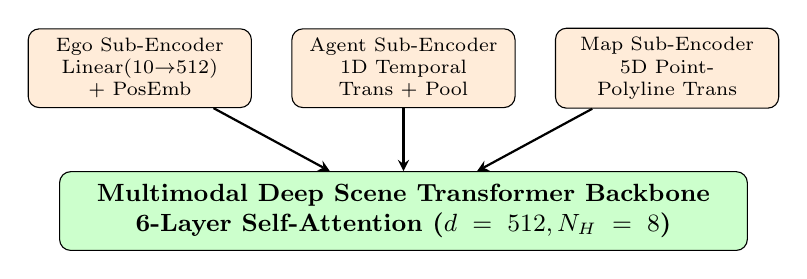
\begin{tikzpicture}[node distance=1.0cm, auto, >=stealth]
        \tikzstyle{sub} = [rectangle, draw, fill=orange!15, text width=2.6cm, text centered, rounded corners, minimum height=1.0cm, font=\scriptsize]
        \tikzstyle{trans} = [rectangle, draw, fill=blue!15, text width=2.6cm, text centered, rounded corners, minimum height=1.0cm, font=\scriptsize\bfseries]
        \tikzstyle{fused} = [rectangle, draw, fill=green!20, text width=8.5cm, text centered, rounded corners, minimum height=1.0cm, font=\small\bfseries]

        \node [sub] (ego) {Ego Sub-Encoder\\Linear(10$\to$512) + PosEmb};
        \node [sub, right=0.5cm of ego] (agent) {Agent Sub-Encoder\\1D Temporal Trans + Pool};
        \node [sub, right=0.5cm of agent] (map) {Map Sub-Encoder\\5D Point-Polyline Trans};

        \node [fused, below=0.8cm of agent] (backbone) {Multimodal Deep Scene Transformer Backbone\\6-Layer Self-Attention ($d=512, N_H=8$)};

        \draw [->, thick] (ego) -- (backbone);
        \draw [->, thick] (agent) -- (backbone);
        \draw [->, thick] (map) -- (backbone);
    \end{tikzpicture}
    }
    \end{center}

    \begin{itemize}
        \item \textbf{Modality Embeddings}: Adds type embeddings ($0: \text{Ego}, 1: \text{Agent}, 2: \text{Map}$) before self-attention fusion.
        \item \textbf{Output}: Sequence of context tokens $C \in \mathbb{R}^{B \times N_{\text{tokens}} \times 512}$ and key padding mask $M_C$.
    \end{itemize}
\end{frame}

\begin{frame}{Sub-Encoder Specifications}
    \begin{block}{1. Ego Trajectory Sub-Encoder}
        $$\mathbf{E}_{\text{ego}} = \mathrm{Linear}_{10 \to 512}(\mathbf{X}_{\text{ego}}) + \mathbf{P}_{\text{ego}} + \mathbf{T}_{\text{type}}(0)$$
        Yields $T_{\text{obs}} = 20$ tokens representing Ego's kinematics.
    \end{block}

    \begin{block}{2. Agent Trajectory Sub-Encoder}
        Processes $N_{\text{ag}}$ surround vessels using a 2-layer 1D Temporal Transformer across time, pooled to 4 temporal sub-tokens per agent ($N_{\text{ag}} \times 4$ total tokens).
    \end{block}

    \begin{block}{3. Map Polyline Sub-Encoder (Point-Polyline Sub-graph)}
        Constructs 5D map features: $[x, y, \Delta x, \Delta y, \text{dist}]$ where $\text{dist} = \sqrt{x^2 + y^2}$.
        Passes through 2-layer Point-Polyline Transformer, adaptive average pooled to 4 spatial tokens per polyline ($N_{\text{map}} \times 4$ total tokens).
    \end{block}
\end{frame}

% ==============================================================================
% SECTION 4: DIFFUSION ACTION DECODER
% ==============================================================================
\section{Diffusion Action Decoder (\texttt{CustomDiT} \& \texttt{DiTBlock})}

\begin{frame}{CustomDiT Diffusion Decoder Architecture}
    \begin{block}{Decoder Core Concept}
        A Diffusion Transformer (\texttt{CustomDiT}) initialized with \texttt{adaLN-Zero} blocks, operating as the trajectory action head.
    \end{block}

    \begin{itemize}
        \item \textbf{Inputs}:
          \begin{itemize}
              \item Noisy action trajectory $x_t \in \mathbb{R}^{B \times 20 \times 4}$ (where actions are $[v_x, v_y, \theta, r]$).
              \item Scalar diffusion timestep $t \in [0, 1]$.
              \item Proprioception vector $y \in \mathbb{R}^{B \times 12}$ (latest Ego status).
              \item Context tokens $C$ and mask $M_C$ from Scene Encoder.
          \end{itemize}
        \item \textbf{Conditioning Vector ($y_{\text{cond}}$)}:
          $$y_{\text{cond}} = \mathrm{TimestepEmbedder}(t) + \mathrm{MlpBlock}_{12 \to 512}(y)$$
    \end{itemize}
\end{frame}

\begin{frame}{\texttt{DiTBlock} \& \texttt{adaLN-Zero} Modulation}
    \begin{block}{Adaptive Layer Normalization (\texttt{adaLN-Zero})}
        Conditioning vector $y_{\text{cond}}$ is passed to a SiLU + Linear layer per block, generating 12 scale/shift/gate parameters:
        $$\begin{pmatrix} \gamma_1, \beta_1, \alpha_1, \dots, \gamma_4, \beta_4, \alpha_4 \end{pmatrix} = \mathrm{Linear}_{512 \to 6144}(\mathrm{SiLU}(y_{\text{cond}}))$$
    \end{block}

    \begin{block}{\texttt{DiTBlock} Forward Computation}
        \begin{align*}
            x_1 &= x + \alpha_1 \cdot \mathrm{SelfAttention}(\mathrm{Modulate}(\mathrm{Norm}_1(x), \beta_1, \gamma_1)) \\
            x_2 &= x_1 + \alpha_2 \cdot \mathrm{MLP}(\mathrm{Modulate}(\mathrm{Norm}_2(x_1), \beta_2, \gamma_2)) \\
            x_3 &= x_2 + \alpha_3 \cdot \mathrm{CustomCrossAttention}(\mathrm{Modulate}(\mathrm{Norm}_3(x_2), \beta_3, \gamma_3), C, M_C) \\
            x_{\text{out}} &= x_3 + \alpha_4 \cdot \mathrm{CrossMLP}(\mathrm{Modulate}(\mathrm{Norm}_4(x_3), \beta_4, \gamma_4))
        \end{align*}
    \end{block}

    \begin{itemize}
        \item \textbf{Zero-Initialization}: Gate parameters $\alpha_i$ are initialized to 0, ensuring blocks act as identity mappings at startup.
    \end{itemize}
\end{frame}

% ==============================================================================
% SECTION 5: MATHEMATICAL FOUNDATIONS & TRAINING PIPELINE
% ==============================================================================
\section{Mathematical Foundations \& Training Pipeline (\texttt{train.py})}

\begin{frame}{Diffusion Loss Space: $\tau_0$-Prediction}
    \begin{block}{Variance-Preserving (VP) Continuous Noise Schedule}
        Forward process diffuses clean velocity actions $\tau_0^v$ into noisy sample $\tau_t^v$:
        $$\tau_t^v = \alpha_t \tau_0^v + \sigma_t \epsilon, \quad \epsilon \sim \mathcal{N}(0, \mathbf{I})$$
        where $\alpha_t = \cos\left(\frac{t + 0.008}{1.008} \frac{\pi}{2}\right)$ and $\sigma_t = \sqrt{1 - \alpha_t^2}$.
    \end{block}

    \begin{alertblock}{Why $\tau_0$-Prediction Beats $\epsilon$-Prediction (HDP Paper Table 1)}
        \begin{itemize}
            \item $\boldsymbol{\epsilon}$\textbf{-Prediction}: Low-noise steps produce high-frequency noise estimation errors, resulting in severe trajectory jitter ($51.07$ score).
            \item $\mathbf{\tau_0}$\textbf{-Prediction}: Directly predicts clean velocity actions $\hat{\tau}_\theta^v = \tau_\theta(x_t, t, C)$. Captures trajectory manifold smoothly ($85.05$ score).
            \item \textbf{Supervised Velocity Loss}:
              $$\mathcal{L}_{\mathrm{vel}} = \mathrm{MSE}(\hat{\tau}_\theta^v, \tau_0^v)$$
        \end{itemize}
    \end{alertblock}
\end{frame}

\begin{frame}{Hybrid Waypoint Loss with Detached Integration}
    \begin{block}{The Dual Representation Principle}
        Velocity prediction ($\tau_0^v$) guarantees smooth kinematics. Integrated position waypoints ($\tau_0^x$) guarantee global spatial precision.
    \end{block}

    \begin{block}{Detached Integration Operator (\texttt{detached\_integral})}
        Truncates gradient backpropagation to sliding window $W=3$ to prevent early velocity components from absorbing all spatial error:
        $$\hat{\tau}_\theta^x = M_W \hat{v}_\theta \cdot \Delta t + \mathrm{sg}\left((M - M_W)\hat{v}_\theta \cdot \Delta t\right) \quad (\Delta t = 10.0\text{s})$$
        where $M$ is lower-triangular integration matrix and $\mathrm{sg}(\cdot)$ is stop-gradient.
    \end{block}

    \begin{block}{Total Training Loss}
        $$\mathcal{L}_{\mathrm{hybrid}} = \mathcal{L}_{\mathrm{vel}} + 0.1 \cdot \mathrm{MSE}(\hat{\tau}_\theta^x, \tau_0^x)$$
        \textbf{Theorem 4.2 Proof}: Preserves score-matching optima while balancing temporal gradient field.
    \end{block}
\end{frame}

\begin{frame}{Training Stabilization: EMA, AMP \& Scheduler}
    \begin{block}{1. Exponential Moving Average (EMA) Weights}
        Maintains smoothed shadow weights $\theta_{\mathrm{EMA}}$ ($\text{decay} = 0.999$):
        $$\theta_{\mathrm{EMA}} \leftarrow 0.999 \cdot \theta_{\mathrm{EMA}} + 0.001 \cdot \theta_{\mathrm{online}}$$
        EMA weights smooth out diffusion loss variance and are saved in checkpoints.
    \end{block}

    \begin{block}{2. Learning Rate Schedule (\texttt{OneCycleLR})}
        5\% linear warmup followed by cosine annealing decay ($5 \times 10^{-4}$ max LR).
    \end{block}

    \begin{block}{3. Automatic Mixed Precision (AMP)}
        Leverages \texttt{torch.amp.autocast("cuda")} and \texttt{torch.amp.GradScaler} for 2x throughput on modern hardware.
    \end{block}
\end{frame}

\begin{frame}{Feature Normalization: Z-Score Standard Normalization}
    \begin{block}{Z-Score Normalization Formula (\texttt{ZScoreNormalizer})}
        Per HDP paper specification, input features and targets are normalized to zero mean and unit variance prior to diffusion:
        $$z = \frac{x - \mu}{\sigma + \epsilon}, \quad \text{Inverse: } x = z \cdot (\sigma + \epsilon) + \mu$$
    \end{block}

    \begin{block}{Feature Channel Normalization Statistics}
        \begin{itemize}
            \item \textbf{Ego/Agent 10D State Features} $[x, y, v_x, v_y, \theta, r, a_{x,\mathrm{ext}}, a_{y,\mathrm{ext}}, \alpha_{\mathrm{ext}}, \beta_{\mathrm{drift}}]$:
              $$\begin{aligned}
              \mu_{\mathrm{state}} &= [0, 0, 3.5, 0, 0, 0, 0, 0, 0, 0] \\
              \sigma_{\mathrm{state}} &= [100.0, 100.0, 3.0, 1.0, 1.0, 0.05, 1.0, 1.0, 0.5, 0.5]
              \end{aligned}$$
            \item \textbf{Coastline Polyline Points} $[x, y]$:
              $$\mu_{\mathrm{map}} = [0, 0], \quad \sigma_{\mathrm{map}} = [2000.0, 2000.0]$$
        \end{itemize}
    \end{block}

    \begin{itemize}
        \item Prevents feature scale dominance (e.g. 2000m coastline coords vs 0.05 rad/s yaw rate).
    \end{itemize}
\end{frame}

% ==============================================================================
% SECTION 6: CPU CLUSTER DISTRIBUTED SCALING
% ==============================================================================
\section{CPU Cluster Distributed Scaling (\texttt{CLUSTER\_SETUP\_GUIDE.md})}

\begin{frame}{Distributed Data Parallel (DDP) for CPU Clusters}
    \begin{block}{PyTorch DDP Cluster Setup}
        Supports scaling across bare-metal CPU nodes without pre-installed packages using PyTorch's \texttt{gloo} backend.
    \end{block}

    \begin{itemize}
        \item \textbf{Launcher}: \texttt{torchrun} across $N$ physical nodes.
        \item \textbf{Backend}: \texttt{backend="gloo"} for CPU clusters (\texttt{"nccl"} for CUDA GPUs).
        \item \textbf{Data Sampler}: \texttt{DistributedSampler(dataset)} partitions dataset equally without duplication.
        \item \textbf{CPU Oversubscription Control}:
          $$\text{OMP\_NUM\_THREADS} = \frac{\text{Physical CPU Cores}}{\text{Processes Per Node}}$$
    \end{itemize}

    \begin{exampleblock}{\texttt{torchrun} Multi-Node Execution Command}
        \texttt{\$ torchrun --nproc\_per\_node=4 --nnodes=2 --node\_rank=0 --master\_addr="192.168.1.100" --master\_port=29500 train.py}
    \end{exampleblock}
\end{frame}

\begin{frame}{Storage Protection \& Zero-Disk-Duplication}
    \begin{alertblock}{The 100GB+ / 500,000 XML Disk Footprint Problem}
        Copying massive scenario datasets to every worker node exhausts local SSD storage and filesystem inodes.
    \end{alertblock}

    \begin{block}{Production Storage Strategies}
        \begin{enumerate}
            \item \textbf{NFS Central Storage (0 GB Worker Footprint)}:
              Download dataset ONCE on Node 0 (Master). Workers mount Master directory via NFS. Workers consume \textbf{0 GB local storage}.
            \item \textbf{In-Memory Zip Streaming}:
              Keep scenarios compressed as \texttt{scenarios.zip}. DataLoader reads XML bytes directly from in-memory zip stream, saving 80\% disk space.
            \item \textbf{Dataset Sharding}:
              Split dataset into $N$ equal chunks so each worker stores only $\frac{1}{N}$ fraction.
        \end{enumerate}
    \end{block}
\end{frame}

% ==============================================================================
% SECTION 7: REINFORCEMENT LEARNING ROADMAP
% ==============================================================================
\section{Reinforcement Learning (HDP-RL) Roadmap}

\begin{frame}{Two-Stage Sequential Training Paradigm}
    \begin{block}{Why Stage 1 (Base Model) Must Precede Stage 2 (RL Fine-Tuning)}
        \begin{itemize}
            \item \textbf{Stage 1 (Pre-training / Base Model)}: Supervised Imitation Learning on real datasets builds multimodal driving priors ($\pi_0$).
            \item \textbf{Stage 2 (Post-training / RL Fine-Tuning)}: Fine-tunes pre-trained base weights using Reward-Weighted Diffusion Loss.
        \end{itemize}
    \end{block}

    \begin{block}{Reward-Weighted Diffusion Loss ($\mathcal{L}_{\mathrm{RL}}$)}
        $$\mathcal{L}_{\mathrm{RL}} = \mathbb{E}_{t, \epsilon, (s, \tau_0) \sim \mathcal{D}} \left[ \exp\left(\beta \cdot \frac{r - \bar{r}}{\sigma_r}\right) \|\hat{\tau}_\theta^v - \tau_0^v\|_P^2 \right]$$
        \begin{itemize}
            \item Group-normalized reward weights score candidate trajectories.
            \item Multi-Reward Function: $r = \lambda_{\text{risk}} r_{\text{risk}} + \lambda_{\text{follow}} r_{\text{follow}} + \lambda_{\text{lane}} r_{\text{lane}}$.
        \end{itemize}
    \end{block}
\end{frame}

% ==============================================================================
% SECTION 8: MODEL PARAMETERS & CONCLUSION
% ==============================================================================
\section{Model Parameters \& Conclusion}

\begin{frame}{Exact Parameter Breakdown ($\sim 86.80\text{M}$ Parameters)}
    \begin{table}
    \centering
    \footnotesize
    \begin{tabular}{llr}
    \toprule
    \textbf{Module Path} & \textbf{Component} & \textbf{Parameter Count} \\
    \midrule
    \texttt{fallback\_encoder} & HighCapacityVectorSceneEncoder & \textbf{27,559,424} \\
    \quad \texttt{ego\_feature\_proj} & Linear(10$\to$512) + PosEmb & $77,696$ \\
    \quad \texttt{agent\_temporal\_trans} & 2-Layer Transformer & $4,204,544$ \\
    \quad \texttt{map\_point\_trans} & 2-Layer Point-Polyline Trans & $4,204,032$ \\
    \quad \texttt{scene\_transformer} & 6-Layer Multimodal Backbone & $18,917,888$ \\
    \midrule
    \texttt{decoder} & CustomDiT Action Decoder & \textbf{59,244,548} \\
    \quad \texttt{t\_embedder} & Timestep MLP & $394,240$ \\
    \quad \texttt{blocks [0..5]} & 6 DiT Blocks with \texttt{adaLN-Zero} & $54,546,432$ \\
    \quad \texttt{final\_layer} & Action Head & $3,149,828$ \\
    \midrule
    \textbf{Total Model} & \textbf{DpVlaModel Backbone} & \textbf{86,803,972 (~86.80M)} \\
    \bottomrule
    \end{tabular}
    \end{table}
\end{frame}

\begin{frame}{Conclusion \& Summary for Clients}
    \begin{block}{Key System Strengths}
        \begin{itemize}
            \item \textbf{Mathematical Rigor}: Physics-consistent body-to-world velocity transforms and score-matching-optimal hybrid loss.
            \item \textbf{Kinematic Smoothness}: $\tau_0$-prediction avoids noise jitter while integrated waypoints preserve spatial precision.
            \item \textbf{Cluster Readiness}: Built-in PyTorch DDP CPU cluster execution with 0-disk-footprint NFS storage architecture.
            \item \textbf{Proven Foundation}: Ready for Stage 2 RL post-training to achieve production-grade maritime autonomy.
        \end{itemize}
    \end{block}
\end{frame}

% ==============================================================================
% Final Slide
% ==============================================================================
\begin{frame}
    \centering
    \vfill
    \Huge \textcolor{MyOrange}{\textbf{Thank You}} \\
    \vspace{0.5cm}
\end{frame}

\end{document}